% Pacotes e configurações padrão do estilo ``article''\
% -------------------------------------
\documentclass[a4paper,11pt]{article}
% Layout
% ------------------------------------------------------------------------------
%     Gráficos e layout ----------------------------------------------------------------------

\ifx\pdfmatch\undefined
\else
    \usepackage[T1]{fontenc}
    \usepackage[utf8]{inputenc}
\fi
% xetex:
\ifx\XeTeXinterchartoks\undefined
\else
    \usepackage{fontspec}
    \defaultfontfeatures{Ligatures=TeX}
\fi
% luatex:
\ifx\directlua\undefined
\else
    \usepackage{fontspec}
\fi
% End engine-specific settings

%      Fonte --------------------------------------------------------------------------------
%\usepackage{lmodern}
\usepackage{times}
%     Pacotes adicionados -------------------------------------------------------------------
\usepackage{ae}
%     Língua e hifenização ------------------------------------------------------------------
\usepackage[portuguese]{babel}
\usepackage{hyphenat}
%      Outros --------------------------------------------------------------------------------
\usepackage{hyperref} % Permite Links personalisados usando hyperref
\usepackage{fancyhdr}
\usepackage{sectsty}
\usepackage{float}   % Gerencia melhor o posicionamento das figuras e tabelas
%\usepackage{graphicx}
\usepackage[pdftex]{color,graphicx}
\usepackage{hyperref}
\usepackage{enumerate} % Permite alterar Layout do enumerate
%\usepackage{pdflscape}  % Permite alterar a orientação da pagina para Paisagem
%\usepackage{ifthen}  % Permite usar condicionais ifelse
%\usepackage[table]{xcolor} % Permite alterar as cores das células de uma tabela
\usepackage{amsmath,amssymb} % Ambiente para uso de elementos matemáticos
\usepackage{caption}
\usepackage{subcaption} % permite o uso de multiplas figuras com legenda (ambiente subfigure)
%\usepackage{minted} % Ambiente minted para colorir código de programas
\usepackage{natbib} % Para referencia bibliográfica
\usepackage{url}    % Referência de links na internet
%\usepackage{listings} % pacote para apresentar código de programação
\usepackage{indentfirst}  % Para indentar o primeiro parágrafo de cada seção
\usepackage{titling}  % Permite Montar uma página de titulo própria

% Layout do documento ------------------------------------------------------------------------
%     Bordas e tamanho da página ------------------------------------------------------------
\usepackage{geometry} 
 \geometry{ % Padrõa ABNT para relatórios
 a4paper,
 left=30mm,
 right=20mm,
 top=30mm,
 bottom=20mm
 }
%     Cabeçalho e Rodapé ---------------------------------------------------------------
\pagestyle{fancy}
  \lhead{}
  \chead{}
  \rhead{}
  \lfoot{}
  \cfoot{}
  \rfoot{\thepage}
%     Númeração ------------------------------------------------------------------------
  \pagenumbering{arabic}
%     Retas do cabeçalho e rodapé ------------------------------------------------------
  \renewcommand{\headrulewidth}{0.5pt}
  \renewcommand{\footrulewidth}{0.5pt}
%     Tamanho da letra de seções e derivadas --------------------------------------------
  \sectionfont{\normalsize}
  \subsectionfont{\small}
%     Hiperlinks ------------------------------------------------------------------------
  \hypersetup{
                  colorlinks,
                  citecolor=black,
                  filecolor=black,
                  linkcolor=black,
                  urlcolor=black
                  }
%     Definições do pdf ----------------------------------------------------------------------
\hypersetup{
    unicode=false,          % non-Latin characters in Acrobat’s bookmarks
    pdftoolbar=true,        % show Acrobat’s toolbar?
    pdfmenubar=true,        % show Acrobat’s menu?
    pdffitwindow=false,     % window fit to page when opened
    pdfstartview={FitH},    % fits the width of the page to the window    
    pdfauthor={Rafael Lima},     % author
    pdfnewwindow=true      % links in new window
}
%     Outros ----------------------------------------------------------------------------
      %\renewcommand{\thesection}{(\alph{section})} % muda o estilo de númeração das sections
      % alterando a formatação dos numeradores de lista de itens
      \renewcommand\theenumi{\arabic{enumi}}
      \renewcommand\labelenumi{(\textit{\theenumi})}
	  \renewcommand\theenumii{\arabic{enumii}}
	  \renewcommand\labelenumii{(\textit{\theenumi.\theenumii})}
      
% ---------------------------------------------------------------------------------------


%\usepackage{circuitikz}
\usepackage[makestderr]{pythontex}

\title{Laboratório 4} % Define o título do Relatório
\author{Rafael Lima}

% Definições Auxiliares ( Macros próprias )
% ------------------------------------------------------------------------------
%\input{relat_aux.tex} % Arquivo com minhas macros
\newcommand{\npy}[1]{\sympy{round(#1,4)}}
% ----------------------------------~>ø<~---------------------------------------
\begin{document}
% Capa e Índice ----------------------------------------------------------------
%--------------------------------------------------- Capa --------------------------------------------
%\newpage
\begin{figure}[h!]
\centering

\includegraphics[scale=0.9]{img/simb_unb.png}
\label{fig:unb}
\end{figure}

\begin{center}
{\LARGE Universidade de Brasília}\\
Departamento de Engenharia Elétrica\\
Professor: Henrique Cezar Ferreira\\
Disciplina: Controle Digital\\
\end{center}


\vspace{0.18\textheight}

\begin{center}
    \Huge \textbf{\\\thetitle \\}
\end{center}

\vspace*{\fill} % Completa espaço em branco e empurra o resto para o final da página

% Tabela com os nome das pessoas do grupo

\begin{table}[H]
    \begin{tabular}{ll}
        % Nome      & Matrícula
        Rafael Lima & 10/0131093 \\
    \end{tabular}
\end{table}

\vspace{0.5cm}

\begin{center}
    \textbf{Brasília\\
    \the\year} % Coloca o Ano atual
\end{center}

\thispagestyle{empty} % Retira o cabeçalho e o rodapé da página

% ------------------------------------------------- Índice -------------------------------------------
\newpage
\tableofcontents
\newpage
% ----------------------------------------------------------------------------------------------------

 % Capa para UnB
% Conteúdo ---------------------------------------------------------------------

\section{Projeto de Controlador na Frequência}

% Código fonte colocado a parte para facilitar validação dentro do ipython
\begin{sympycode}
# Get Source Code
sys.path.insert(1, '../../')
from src.python.exsim4 import *
\end{sympycode}

\subsection{Transformada z de G(s) com segurador de ordem zero em série}

A discretização pode ser aproximada aplicando-se a transformada z em conjunto de um segurador de ordem zero em série com o sistema. desta forma temos $G_{ho}(z) = Z(G_{zoh}(s)G(s)$ onde $G_{zoh}(s) = \frac{1-e^{-ts}}{s}$. aplicando as propriedades da transformada z:

$$
\begin{array}{lcl}
    Z(\frac{1-e^{-ts}}{s}G(z)) &=& Z(\frac{1}{s}G(z)) - Z(\frac{e^{-ts}}{s}G(z))\\
    &=& z(\frac{1}{s}G(z)) - (z^{-1})Z(\frac{1}{s}G(z))\\
    &=& (1 - z^{-1})Z(\frac{1}{s}G(z))\\
    &=& (1 - z^{-1})Z(\sympy{(1/s)*sG})\\
\end{array}
$$

para facilitar o cálculo, fatorando o termo $\sympy{(1/s)*sG}$ pelo método de frações parciais:

\begin{equation}\label{eq:ex4-partialfrac}
\frac{G(s)}{s} = \frac{1}{s+1}-\frac{1}{s}+\frac{1}{s^2}
\end{equation}

pela tabela, temos que a transformada z de \ref{eq:ex4-partialfrac} é

$$G(z) = \sympy{sGz}$$
$$G(z) = \sympy{sGz.combsimp()}$$

logo, substituindo $t = \sympy{nT}$ e simplificando temos:

\begin{equation}
    G(z) = \sympy{roundExpr(sGz.combsimp().subs(T,nT))}
\end{equation}

\subsection{Transformada w}

Substituindo $z = \sympy{zw}$

$$
G(w) = G(z)|_{z=\sympy{zw}} = \sympy{sGw}
$$

substituindo $t = \sympy{nT}$ e simplificando temos

\begin{equation}
    G(w) = \sympy{roundExpr(sGw.combsimp().subs(T,nT))}
\end{equation}

\subsection{Calculo ganho planta}

$$E_v = lim_{w \rightarrow 0}\ w G(w)$$
$$E_v = lim_{w \rightarrow 0}\  \sympy{w*(sGw.combsimp())}$$
$$E_v = lim_{w \rightarrow 0}\  \sympy{exprLimEv}$$
$$E_v = \sympy{Ev}$$

Como $K_v = \frac{1}{E_v} = \sympy{1/Ev}$  e $K_v = 2$ então $K = \sympy{nK}$

\subsection{Diagrama de Bode}

\begin{figure}[H]
    \centering
    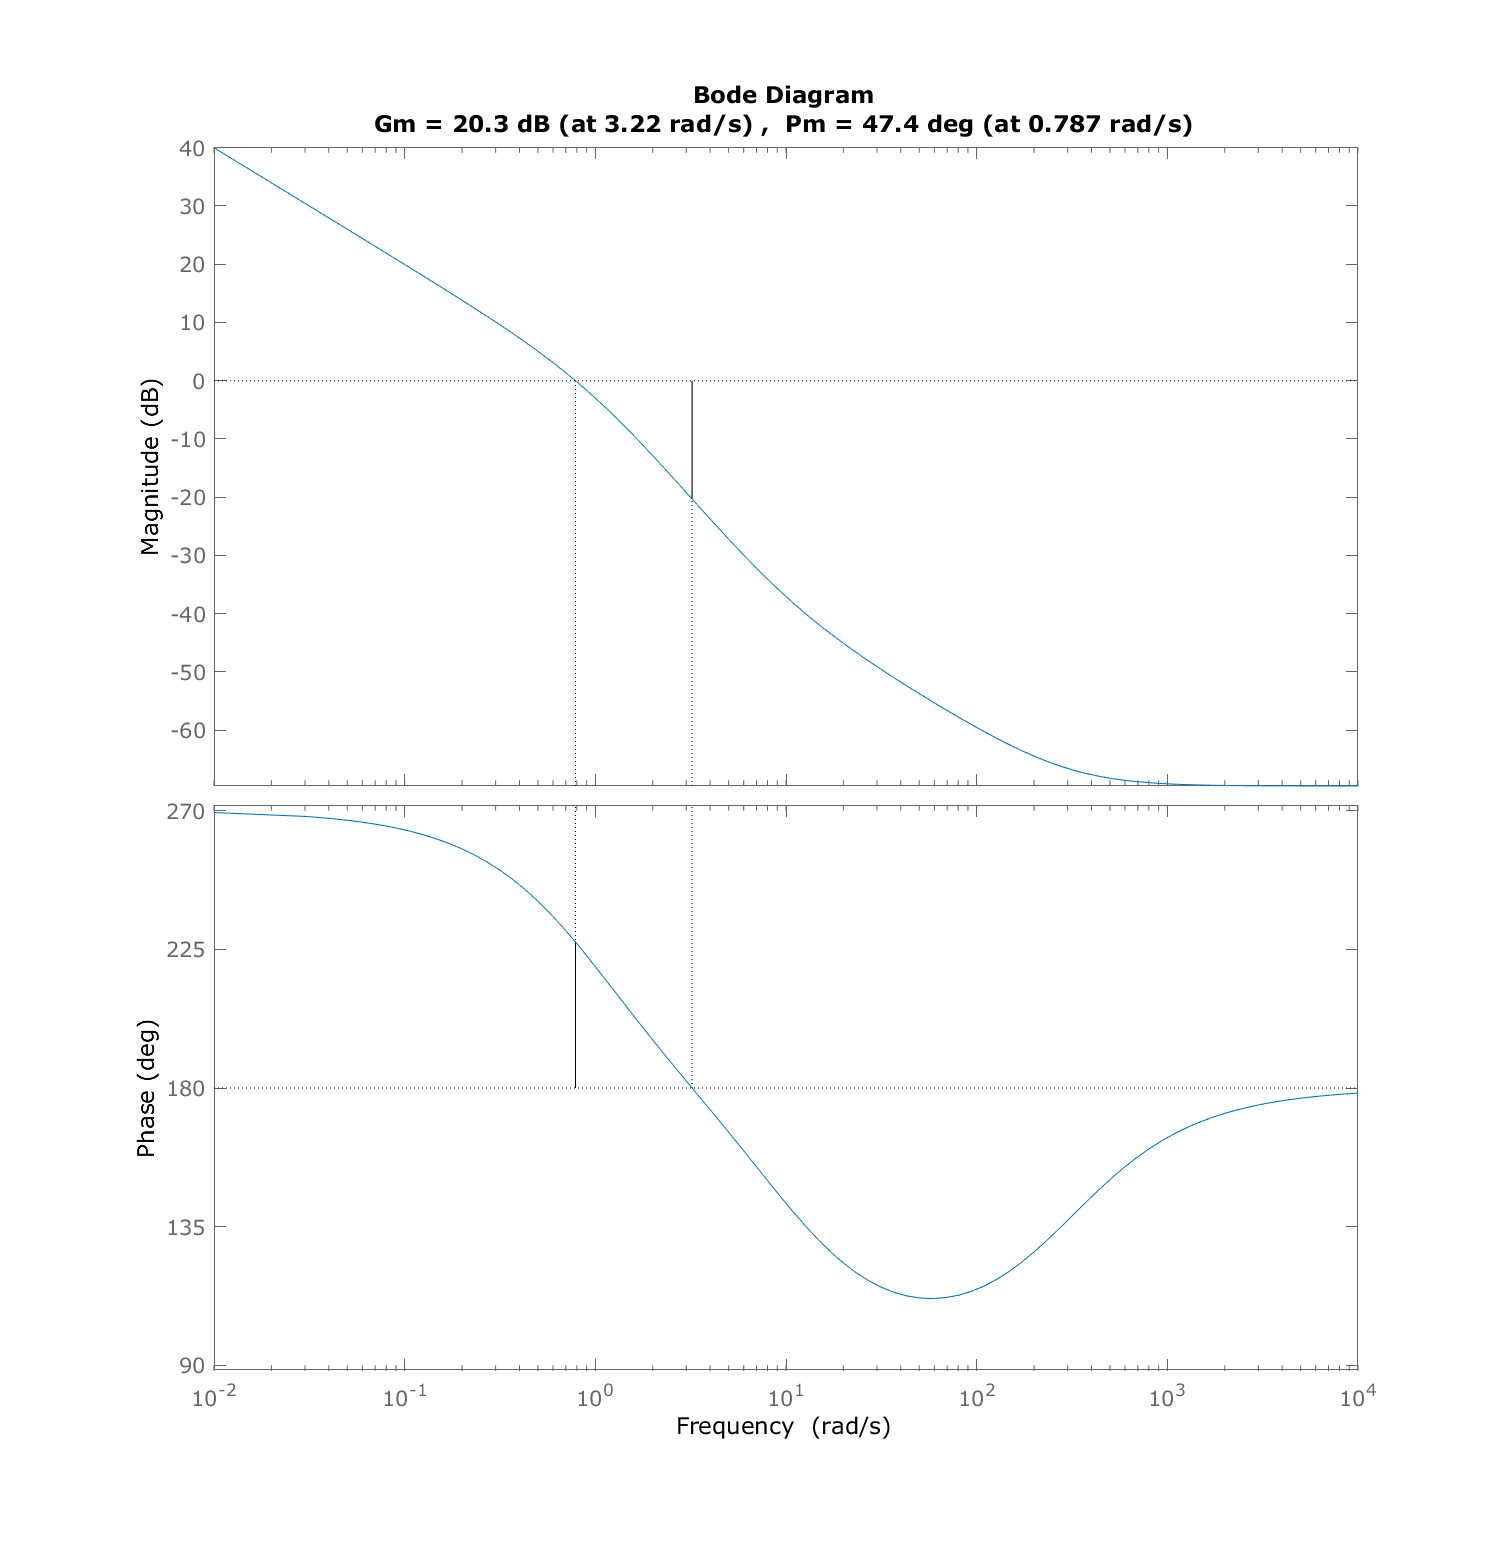
\includegraphics[width=0.9\linewidth]{img/exsim4-bodeplot-gw.png}
    \caption{Diagrama de Bode para $G(w)$}
\end{figure}

\section{Conclusão}


% ------------------------------------------------------------------------------
\newpage
% Referências
\addcontentsline{toc}{section}{Referências} % Adiciona linha no indice
\bibliographystyle{abbrv} % Define Estilo e gera bibliografia
\bibliography{references} % Adiciona Arquivo com Referências

% Acrescentadas no arquivo references.bib
% para usa-las no texto basta usar \citep{}
% para citar sem usar no texto basta usar \nocite{}
\nocite{sympy}
\nocite{pythontex}
\nocite{matlabcontrol}
\nocite{matlabsymbolic}

% ------------------------------------------------------------------------------
\newpage
\section*{Anexos}
\addcontentsline{toc}{section}{Anexos} % Adiciona linha no indice
%\subsection*{Python}

%Para os cálculos e demonstrações foi utilizado o pacote \textit{Python}\TeX\ \cite{pythontex} para o \LaTeX\ em conjunto da bibliteca \textit{sympy}\cite{sympy}. Segue o script completo em python:

%\inputminted[xleftmargin=15pt,linenos,frame=single,framesep=5pt,breaklines=true]{python}{../python/exsim4.py}

\newpage
\subsection*{Matlab}

%\subsubsection*{Parte 1}
Para o desenho dos gráficos e simulações foi utilizado o \textit{Matlab} em conjunto das toolbox \textit{Control System}\cite{matlabcontrol} e \textit{Symbolic Math}\cite{matlabsymbolic}. Segue o código referente usado

\inputminted[xleftmargin=15pt,linenos,frame=single,framesep=5pt,breaklines=true]{matlab}{../matlab/exsim4/exsim4.m}

%\subsubsection*{Parte 2}
%Na segunda parte foi utilizado uma versão modificada do script em \textit{Matlab} fornecido pelo professor:
%\inputminted[xleftmargin=15pt,linenos,frame=single,framesep=5pt]{matlab}{../matlab/exsim2/exsim2script.m}



% ------------------------------------------------------------------------------
\end{document}
